\part{Background}
\label{part:background}

%======================================================================
\chapter{Physics at the mesoscale}
\label{ch:swimming at the mesoscale}

\markright{Swimming at the mesoscale}
%======================================================================

\section{Low Renolds number regime}
\label{st:lowreynoldsnumber}

At the mesoscale, where objects such as bacteria and colloidal particles operate, the physical world is governed by a regime in which viscous forces dominate over inertial ones. This regime is characterized by a small Reynolds number (Re), a dimensionless quantity that compares inertial to viscous effects. Therefore, the force applied at that moment will describe the movement or displacement performed, not deppending on any past force, this is a characteristic of an overdamped system. In his seminal lecture, Life at Low Reynolds Number, Purcell highlighted the surprising and often counterintuitive behaviors that emerge in such environments~\cite{purcell2014life}. For instance, time-reversible motion — common at macroscopic scales — is ineffective for propulsion at low Re, necessitating non-reciprocal strategies like flagellar rotation or body undulation. This leads to the scallop theorem, that states that an animal with such degrees of freedom — in a viscous regime — will not have a net displacement. 

This whole process can be described by the Navier-Stokes equation without the inertia terms, leaving us without any time deppending terms as shown in Eq. (\ref{eq:Navier-Stokes}). 

\begin{equation}
  - \nabla p + \eta \nabla ^2 \vec{v} = 0
  \label{eq:Navier-Stokes}
\end{equation}

This has been a topic of interest for researchers that are constantly looking for ways of transportation in those environments for specific tasks. Unfortunately this is not the only challenge we face when moving at the microscale.

\section{Brownian Motion and Thermal Fluctuations}
\label{st:brownianmotion}

Even though this is a viscous regime, particles are not static. At small length scales, such as those of colloidal particles or bacteria, random thermal fluctuations become a dominant source of motion. This phenomenon, known as \textit{Brownian motion}, was first explained quantitatively by Albert Einstein in 1905. He demonstrated that the irregular paths observed in microscopic particles suspended in fluid result from collisions with the molecules of the surrounding medium~\cite{einstein1906theory}.

Einstein's work provided one of the first convincing arguments for the molecular nature of matter and led to a mathematical description of how these random movements accumulate over time. Specifically, he derived that the mean squared displacement (MSD) of a particle grows linearly with time:

\begin{equation}
  \langle x^2(t) \rangle = 2Dt\text{,}
  \label{eq:msd}
\end{equation}

where $D$ is the diffusion coefficient, a measure of how quickly particles spread out. Einstein further related this coefficient to measurable physical parameters through the expression:

\begin{equation}
  D = \frac{k_{B}T}{6\pi \eta R}\text{,}
  \label{eq:diffusioncoefficient}
\end{equation}

where $k_B$ is Boltzmann’s constant, $T$ the absolute temperature, $\eta$ the dynamic viscosity of the fluid, and $R$ the radius of the spherical particle. This relation — often referred to as the \textit{Einstein-Stokes equation} — is foundational in soft matter and colloidal physics.

In the systems considered in this thesis, Brownian motion plays a crucial role in the dynamics of passive colloids and must be accounted for even in the presence of external fields or active agents, such as bacteria.

\vspace{1em}

While Einstein’s formulation captures the long-term diffusive behavior of Brownian particles, it does not account for their instantaneous dynamics. To describe how particles move under both viscous damping and random thermal forces, we turn to a stochastic differential equation known as the \textit{Langevin equation}.

\subsection{Stochastic Representation}
\label{stochasticrepresentation}

The Langevin equation \cite{uhlenbeck1930theory} in one dimension, including inertial effects, damping, and thermal noise, can be written as:

\begin{equation}
  m\ddot{x} = F - \lambda \dot{x} + \eta(t)\text{,}
  \label{eq:newton}
\end{equation}

where $m$ is the particle mass, $\lambda$ is the damping coefficient, and $\eta(t)$ is a stochastic force representing thermal noise. For simplicity, we write the velocity as $v = \dot{x}$, leading to:

\begin{equation}
  m\frac{dv}{dt} = F - \lambda v + \eta(t)\text{.}
  \label{eq:newtonv}
\end{equation}

Discretizing time with a small step $dt$, we apply the definition of a derivative:

\begin{equation}
  m \frac{v(t + dt) - v(t)}{dt} = F - \lambda v(t) + \eta(t)\text{.}
  \label{eq:newtonderivative}
\end{equation}

The thermal noise term $\eta(t)$ is modeled as a Gaussian white noise process:

\begin{equation}
  \eta(t)\, dt = g\, dW\text{,}
  \label{eq:eta}
\end{equation}

where $dW$ is a Wiener process (increment of Brownian motion) such that:

\begin{equation}
  \langle dW \rangle = 0\,, \quad \langle dW^2 \rangle = dt\text{.}
  \label{eq:meanvariance}
\end{equation}

Solving for $v(t + dt)$ gives:

\begin{equation}
  v(t + dt) = v(t) + \frac{dt}{m}(F - \lambda v(t)) + g\, dW\text{.}
  \label{eq:velocityplusone}
\end{equation}

Now, assuming no deterministic force ($F = 0$) — as is the case for free passive particles:

\begin{equation}
  v(t + dt) = v(t) - \frac{\lambda dt}{m} v(t) + g\, dW\text{.}
  \label{eq:noforce}
\end{equation}

Taking the expectation value (mean) of both sides:

\begin{equation}
  \langle v(t + dt) \rangle = \langle v(t) \rangle - \frac{\lambda dt}{m} \langle v(t) \rangle + g \langle dW \rangle\text{.}
  \label{eq:mean}
\end{equation}

Since $\langle dW \rangle = 0$, the last term vanishes:

\begin{equation}
  \langle v(t + dt) \rangle = \langle v(t) \rangle \left( 1 - \frac{\lambda dt}{m} \right)\text{.}
\end{equation}

In the limit of small $dt$, this leads to the differential equation:

\begin{equation}
  \frac{d}{dt} \langle v(t) \rangle = - \frac{\lambda}{m} \langle v(t) \rangle\text{,}
  \label{eq:derivative}
\end{equation}

whose solution is:

\begin{equation}
  \langle v(t) \rangle = \langle v(0) \rangle\, e^{-\lambda t / m}\text{.}
\end{equation}

This result shows that the average velocity of a particle in a viscous fluid decays exponentially due to damping. The characteristic timescale $\tau = m/\lambda$ describes how quickly the particle forgets its initial velocity, after which the motion becomes diffusive.

%%%%

\subsection{Velocity Statistics and Energy Equipartition}

To compute the variance of the velocity, we start again from the Langevin equation in discretized form, without external forces:

\begin{equation}
  v(t + dt) = v(t) - \frac{\lambda}{m} v(t) dt + \frac{g}{m} dW \text{.}
\end{equation}

Squaring both sides:

\begin{align}
  v(t + dt)^2 &= \left[ v(t) - \frac{\lambda}{m} v(t) dt + \frac{g}{m} dW \right]^2 \text{,}\\
              &= v(t)^2 + \left( \frac{\lambda}{m} \right)^2 v(t)^2 dt^2 + \left( \frac{g}{m} \right)^2 dW^2 \nonumber \\
              &\quad - 2 \frac{\lambda}{m} v(t)^2 dt + 2 \frac{g}{m} v(t) dW - 2 \frac{\lambda g}{m^2} v(t) dW \text{.}
\end{align}

Now we take the expectation value:

\begin{align}
  \langle v(t + dt)^2 \rangle &= \langle v(t)^2 \rangle + \left( \frac{\lambda}{m} \right)^2 \langle v(t)^2 \rangle dt^2 + \left( \frac{g}{m} \right)^2 \langle dW^2 \rangle \nonumber \\
                              &\quad - 2 \frac{\lambda}{m} \langle v(t)^2 \rangle dt + 2 \frac{g}{m} \langle v(t) \rangle \langle dW \rangle - 2 \frac{\lambda g}{m^2} \langle v(t) \rangle \langle dW \rangle \text{.}
\end{align}

Using the properties of the Wiener process:

\[
  \langle dW \rangle = 0, \quad \langle dW^2 \rangle = dt \text{.}
\]

And neglecting second-order small terms (\( dt^2 \)), we obtain:

\begin{equation}
  \langle v(t + dt)^2 \rangle = \langle v(t)^2 \rangle + \frac{g^2}{m^2} dt - 2 \frac{\lambda}{m} \langle v(t)^2 \rangle dt \text{.}
\end{equation}

Taking the continuous limit:

\begin{equation}
  \frac{d}{dt} \langle v(t)^2 \rangle = -2 \frac{\lambda}{m} \langle v(t)^2 \rangle + \frac{g^2}{m^2} \text{.}
\end{equation}

This is a linear first-order ODE. Solving it with variation of constants yields:

\begin{equation}
  \langle v(t)^2 \rangle = \frac{g^2}{2 \lambda m} + D e^{-2 \lambda t / m} \text{.}
\end{equation}

As \( t \to \infty \), the exponential term vanishes and we get the stationary value:

\begin{equation}
  \langle v(\infty)^2 \rangle = \frac{g^2}{2 \lambda m} \text{.}
\end{equation}

From the equipartition theorem, we know that the average kinetic energy is:

\[
  \frac{1}{2} m \langle v^2 \rangle = \frac{1}{2} k_B T \text{.}
\]

Therefore:

\begin{equation}
  \langle v^2 \rangle = \frac{k_B T}{m} \text{.}
\end{equation}

Matching this to our stochastic result:

\begin{equation}
  \frac{k_B T}{m} = \frac{g^2}{2 \lambda m} \quad \Rightarrow \quad g^2 = 2 \lambda k_B T, \quad g = \sqrt{2 \lambda k_B T} \text{.}
\end{equation}

This defines the noise amplitude in terms of temperature, viscosity, and Boltzmann’s constant.

\subsection{Overdamped Dynamics and Diffussion}

In the overdamped limit, inertia is negligible, so the Langevin equation becomes:

\begin{equation}
  0 = F - \lambda \frac{dx}{dt} + \eta(t) \text{.}
\end{equation}

Solving for the velocity:

\begin{equation}
  \frac{dx}{dt} = \frac{1}{\lambda} (F + \eta(t)) \text{.}
\end{equation}

For free diffusion (\( F = 0 \)):

\begin{equation}
  \frac{dx}{dt} = \frac{1}{\lambda} \eta(t) \text{.}
\end{equation}

Using stochastic calculus with \( \eta(t) dt = g dW \), we write:

\begin{equation}
  x(t + dt) = x(t) + \frac{g}{\lambda} dW \text{.}
\end{equation}

\paragraph{Mean Position}

Taking the expectation:

\begin{equation}
  \langle x(t + dt) \rangle = \langle x(t) \rangle + \frac{g}{\lambda} \langle dW \rangle = \langle x(t) \rangle \text{.}
\end{equation}

So the mean position remains constant in free diffusion.

\paragraph{Mean Square Displacement (MSD)}

Squaring the position update:

\begin{equation}
  x(t + dt)^2 = x(t)^2 + 2 \frac{g}{\lambda} x(t) dW + \left( \frac{g}{\lambda} \right)^2 dW^2 \text{.}
\end{equation}

Taking the expectation:

\begin{align}
  \langle x(t + dt)^2 \rangle &= \langle x(t)^2 \rangle + 2 \frac{g}{\lambda} \langle x(t) \rangle \langle dW \rangle + \frac{g^2}{\lambda^2} \langle dW^2 \rangle \text{,}\\
  &= \langle x(t)^2 \rangle + \frac{g^2}{\lambda^2} dt \text{.}
\end{align}

In differential form:

\begin{equation}
  \frac{d}{dt} \langle x(t)^2 \rangle = \frac{g^2}{\lambda^2} \text{.}
\end{equation}

Using \( g^2 = 2 \lambda k_B T \), we substitute:

\begin{equation}
  \frac{d}{dt} \langle x(t)^2 \rangle = \frac{2 k_B T}{\lambda} \text{.}
\end{equation}

Integrating gives the mean squared displacement (MSD):

\begin{equation}
  \langle x(t)^2 \rangle = \frac{2 k_B T}{\lambda} t \text{.}
\end{equation}

This is the classical diffusion result, where the diffusion coefficient is \( D = \frac{k_B T}{\lambda} \), consistent with Einstein's expression.



%%%%
%This raises a fundamental question: Can these fluctuations be harnessed to perform useful work? This idea lies at the heart of thought experiments such as the Feynman ratchet, which challenge our understanding of thermodynamics at microscopic scales.


\begin{figure}[H]
  \begin{center}
    \includegraphics[width=0.8\textwidth]{figures/passivebrowniantrajectorymsd.pdf}
  \end{center}
  \caption[Example of brownian motion]{A colloidal particle undergoes random, thermally induced displacements in a fluid medium. \textbf{Panel a)} shows the trajectory of the particle. \textbf{ Panel b)} shows the corresponding mean squared displacement (MSD) as a function of time, illustrating the linear relationship predicted by Einstein for diffusive behavior (orange) and the one obtained through a numerical simulation (blue).}\label{fig:passivebrowniantrajectory}
\end{figure}

\chapter{Ratchets and Rectification Mechanisms}
\label{ch:ratchetsandrectificationmechanisms}

\section{The Feynman-Smoluchowski ratchet}

The inherent randomness of Brownian motion naturally leads to the question: can this disorder be transformed into order? In other words, can the random thermal motion of particles be used to produce directed movement or extract work? This question sits at the core of statistical mechanics and was famously explored by Richard Feynman in his lectures on physics, through a thought experiment known as the Feynman ratchet and pawl~\cite{feynman1963feynman}.

The Feynman ratchet consists of a set of vanes connected to a ratchet wheel, immersed in a fluid (Fig.~\ref{fig:feynmanratchet}). The idea is: random collisions from the surrounding molecules could push the vanes, but the pawl only allows rotation in one direction. At first glance, this asymmetric mechanism seems capable of converting random thermal motion into unidirectional rotation, apparently violating the second law of thermodynamics.

\begin{figure}
  \begin{center}
    \includegraphics[width=0.65\textwidth]{figures/feynmanratchet.png}
  \end{center}
  \caption[Feynman ratchet]{Visual representation of the Feynman ratchet. Obtained from \cite{feynman1963feynman}}\label{fig:feynmanratchet}
\end{figure}


However, Feynman's analysis showed that when both the ratchet and the pawl are in thermal equilibrium with the same heat bath, the system cannot produce net work. The pawl itself undergoes thermal fluctuations and can occasionally lift off, allowing the ratchet to move backward. Over time, the forward and backward movements average out, and no net rotation occurs. This result reinforces the principle that thermal fluctuations alone cannot be rectified to perform work without a temperature gradient or an external energy input.

\begin{table}[ht]
\centering
\renewcommand{\arraystretch}{1.4}
\caption[Summary of operation of ratchet and pawl.]{Summary of operation of ratchet and pawl. Obtained from \cite{feynman1963feynman}}
\label{tab:ratchet_pawl}
\begin{tabular}{>{\itshape}l l l}
\toprule
\textbf{Forward:} & Needs energy & $\epsilon + L \theta$ from vane. \quad $\therefore$ Rate = $\dfrac{1}{\tau} e^{-(L\theta + \epsilon)/kT_1}$ \\
                  & Takes from vane & $L\theta + \epsilon$ \\
                  & Does work & $L\theta$ \\
                  & Gives to ratchet & $\epsilon$ \\
\midrule
\textbf{Backward:} & Needs energy & $\epsilon$ for pawl. \quad $\therefore$ Rate = $\dfrac{1}{\tau} e^{-\epsilon/kT_2}$ \\
                   & Takes from ratchet & $\epsilon$ \\
                   & Releases work & $L\theta$ \\
                   & Gives to vane & $L\theta + \epsilon$ \\
\bottomrule
\end{tabular}

\vspace{1em}
If system is reversible, rates are equal, hence 
\[
\frac{\epsilon + L\theta}{T_1} = \frac{\epsilon}{T_2}.
\]
\[
\frac{\text{Heat to ratchet}}{\text{Heat from vane}} = \frac{\epsilon}{L\theta + \epsilon}.
\quad \text{Hence} \quad \frac{Q_2}{Q_1} = \frac{T_2}{T_1}.
\]
\end{table}

Despite this limitation, the Feynman ratchet introduced a powerful concept: asymmetry combined with non-equilibrium conditions can, in principle, produce directed motion. This idea is foundational in the study of Brownian motors, biomolecular machines, and active matter systems, including the systems explored in this thesis. In such systems, energy is continuously supplied, whether through bacterial metabolism or magnetic field modulation, creating the necessary non-equilibrium environment that allows motion rectification to occur.

The failure of the Feynman ratchet in thermal equilibrium is intimately connected to another famous thought experiment: Maxwell's demon. Both systems attempt to extract work from thermal fluctuations through selective processes—the ratchet through mechanical asymmetry, and the demon through information gathering.

Maxwell's demon, proposed in 1867, imagines a microscopic being that can sort fast and slow molecules between two chambers, creating a temperature difference without apparent work. Similarly, the pawl in Feynman's ratchet acts as a mechanical "demon," attempting to select only forward fluctuations while blocking backward motion. However, both fail for the same fundamental reason: the cost of selection itself~\cite{maxwell1871theory, maxwell1867letter}.

Brillouin (1951) and later Landauer (1961) showed that Maxwell's demon must expend energy to measure molecular velocities and erase information, with the minimum energy cost being $kT\ln{2}$ per bit erased. In the Feynman ratchet, the pawl must "decide" whether to allow motion, and this decision-making process—manifested as thermal fluctuations of the pawl itself—has an entropic cost that exactly cancels any work extracted~\cite{brillouin1951maxwell, landauer1961irreversibility}.

This connection reveals a deep principle: rectification requires either an information gradient (knowledge about the system) or an energy gradient (non-equilibrium conditions). As Parrondo and Español (1996) demonstrated, the Feynman ratchet can be viewed as an information engine where the pawl performs measurements on the ratchet's position. When the pawl and ratchet are at the same temperature, the information gained equals the entropy produced, yielding no net work~\cite{parrondo1996criticism}.


\section{Brownian ratchets}
\label{sct:brownianratchets}

While Feynman's ratchet fails due to thermal equilibrium, rectified motion becomes possible when detailed balance is broken through external driving. Magnasco (1993) demonstrated this principle through the "rocking ratchet" mechanism~\cite{magnasco1993forced}. In his model, a Brownian particle moves in an asymmetric periodic potential—essentially a sawtooth-shaped energy landscape with gentle slopes in one direction and steep walls in the other.
The crucial innovation was applying an oscillating force $F(t) = A\cos(\omega t)$ that rocks the potential back and forth. Although this force has zero time average—pushing equally left and right—the combination with the spatial asymmetry produces net directional motion. When the force tilts the potential forward, particles easily climb the gentle slopes and can overcome barriers. When tilted backward, particles encounter steep walls and remain trapped. This asymmetric response to symmetric driving breaks the forward-backward symmetry of thermal diffusion.

This mechanism differs fundamentally from Feynman's original ratchet: rather than attempting to rectify equilibrium fluctuations (which violates the second law), the rocking ratchet continuously injects energy through the oscillating force. The time-dependent driving maintains the system far from equilibrium, enabling the spatial asymmetry to generate directed transport. This principle—that asymmetry plus non-equilibrium driving yields rectification—underlies numerous biological processes and provides the theoretical foundation for the magnetically-driven ratchets explored in this thesis.

\begin{figure}[h]
  \begin{center}
    \includegraphics[width=0.95\textwidth]{figures/ratchet_potential.png}
  \end{center}
  \caption[Ratchet potential example.]{Example of a commonly used ratchet potential.}\label{fig:}
\end{figure}


Following Magnasco's rocking ratchet where an oscillating force drives particles in a static potential, Ajdari et al. (1994) analyzed rectification in periodic structures with either spatial or temporal asymmetry~\cite{ajdari1994rectified}. Using a sawtooth potential with asymmetric slopes (steep of height $\epsilon/a$ and gentle of $\epsilon/b$), they identified distinct transport regimes as a function of the AC force amplitude $\gamma$. 

For small forces $\gamma < \epsilon/a$, particles remain trapped. In the intermediate regime $\epsilon/a < \gamma < \epsilon/b$, rectification occurs as particles can climb the gentle slope but not the steep one, yielding either integer velocities $V = n$ when particles fully relax between cycles, or rational velocities $V = n - 1/(m+1)$ when incomplete relaxation creates a periodic pattern over multiple cycles.


This concept was later demonstrated experimentally by Faucheux et al. (1995), who created an "optical thermal ratchet" using focused laser beams~\cite{faucheux1995optical}. To generate a circular trap without introducing external forces, they passed the laser through a plate to create circular polarization, maintaining constant laser intensity along the circular path. By rotating the laser frequency fast enough, particles could not experience any directed force from the beam itself, allowing them to move freely, then modulated the beam intensity to create an asymmetric potential mimicking a ratchet shape, as shown in Figure~\ref{fig:faucheuxexperiment}. They observed that particles localized in potential minima when the modulation was turned on, while for sufficiently long periods, particles moved either backward or forward with equal probability.

\begin{figure}[h]
  \begin{center}
    \includegraphics[width=0.65\textwidth]{figures/FaucheuxExperiment.png}
  \end{center}
  \caption[Optical thermal ratchet by Faucheux]{When the modulation is on, the beam intensity follows the shape of a ratchet potential with 4 periods per cycle. When the modulation is off, the intensity remains constant, allowing particles to diffuse freely. Obtained from~\cite{faucheux1995optical}.}\label{fig:faucheuxexperiment}
\end{figure}

A different approach was developed by Lee et al. (2004), who employed holographic optical trapping with a symmetric potential~\cite{lee2005observation}. Their system consisted of discrete optical tweezers functioning as potential wells. Between each state, particles are released and free to diffuse, nevertheless they can rapidly jump between adjacent traps. Using this methodology, they achieved net particle displacement in one direction, as illustrated in Figure~\ref{fig:deterministicthermalratchet}. Remarkably, when they reversed the direction of well displacement, particles followed the trap movement in the opposite direction. Due to this predictable response to trap motion, they named this system a "deterministic thermal ratchet."


 \begin{figure}[h]
  \begin{center}
    \includegraphics[width=0.30\textwidth]{figures/DeterministicThermalRatchet.png}
  \end{center}
  \caption[Deterministic thermal ratchet by Lee et al.]{Discrete pattern of optical traps with displacement in one directio, minimum width of $\sigma$ and a maximum width of $L$. Obtained from~\cite{lee2005observation}}\label{fig:deterministicthermalratchet}
 \end{figure}

 Lebedev et al. (2009) modified this approach by using three linearly polarized beams acting only in the xy-plane, as shown in Figure~\ref{fig:lebedevexperiment}~\cite{lebedev2009two}. They applied forces to particles by phase-modulating two of the three lasers, which shifts the entire optical lattice. The modulation was generated using RF generators to produce potentials $V_x$ and $V_y$. The sum $V_x + V_y$ served as the input signal for beam 2, while the difference $V_x - V_y$ was used for beam 3, creating the rocking forces. They studied this system using ultracold rubidium atoms as test particles. To track the atomic positions, they employed a CCD camera to determine the center of mass of the atomic cloud.

 In their first experiment, they applied a biharmonic drive along only one axis. As expected, the system reduced to a one-dimensional harmonic ratchet, and they observed directed particle motion along the axis of the applied biharmonic force. In subsequent experiments, they applied harmonic drives along both axes, with one frequency being twice the other. Their results showed that particles experienced directed motion along the axis with the faster harmonic, while motion along the other axis remained diffusive. In their final experiment, they applied biharmonic drives simultaneously along both axes to investigate whether directed transport could be achieved in two dimensions. By varying the relative weights of the forces along each axis, they demonstrated that it was possible to control the atomic displacement and direct atoms to specific target positions as shown in Figure~\ref{fig:lebedevexperiment} a).


 \begin{figure}[h]
  \begin{center}
    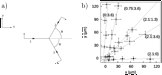
\includegraphics[width=0.80\textwidth]{figures/LebedevExperiment.png}
  \end{center}
  \caption[Lebedev experiment.]{\textbf{Panel a)} Lattice beam configuration in the xy plane. $\theta$ = 60°. \textbf{Panel b)} Position of the atomic cloud center of mass at different instants and forces when applying biharmonic at ehe same time in xy-plane. Obtained from~\cite{lebedev2009two}.}\label{fig:lebedevexperiment}
 \end{figure}


 Following the same lattice-based approach, Arzola et al. (2017) successfully recreated all five two-dimensional Bravais lattices using computer-generated holographic optical micromanipulation~\cite{arzola2017omnidirectional}. Their potential consisted of Gaussian wells distributed along a primary lattice, combined with a shifted replica of the same lattice with a reduced depth factor, Q, compared to the original. The asymmetry of the resulting potential depended directly on both the depth factor Q and the displacement between the original and replica lattices. They implemented the rocking mechanism by moving the particle cell along one axis.

The researchers performed three main experiments to validate their results, each with three different diffusion parameters (including no diffusion as one condition), calculating the current in the x and y axes with respect to the amplitude of movement. In the first experiment, they set the asymmetry parallel to the rocking force. They observed that since the wells were aligned with the particle movement, particles tended to move in the direction of the force, traveling from well to well, while experiencing no movement in the perpendicular direction. Current was present along the entire amplitude range.

The second experiment positioned the asymmetry perpendicular to the rocking force direction, yielding interesting results. Similar to the first experiment, current appeared along only one axis (the asymmetry axis), but the current behaved like a Gaussian bell curve. When the rocking movement amplitude approached the asymmetry lattice spacing, particles only moved back and forth between two wells in the x direction, experiencing no current in the y axis.

For the final experiment, they examined how the system behaved under a combination of both previous configurations. They created an oblique lattice with the asymmetry aligned with the rocking force direction, producing an oblique particle current. The results were essentially a combination of the two previous experiments: at certain amplitudes, current appeared in both axes, but as amplitude increased, the y-axis current decreased while the x-axis current increased. The results for each experiment can be seen in Figure~\ref{fig:arzolaexperiment}.

\begin{figure}[h]
  \begin{center}
    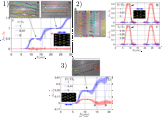
\includegraphics[width=0.65\textwidth]{figures/ArzolaExperiment.png}
  \end{center}
  \caption[Arzola experiment.]{\textbf{Panel 1)} Experimental trajectories for  assymetry parallel to rocking movement with a) rocking amplitud of 13 $\mu$m and b) 23 $\mu$m.c) Graphs of simulations showing the current for each axis. \textbf{Panel 2)} Experimental trajectories for assymetry perpendicular to rocking movement with a) rocking amplitud of 10 $\mu$m. b) and c) Shows the current for each axis with different lattice parameters. \textbf{Panel 3)} Experimental trajectories for oblique lattice with assymetry perpendicular to the rocking movement with a) rocking amplitud of 11$\mu$m. b) Current for each axis. Obtained from~\cite{arzola2017omnidirectional}.}\label{fig:arzolaexperiment}
\end{figure}

Feynman demonstrated that a purely thermal Brownian ratchet cannot generate directed motion due to the second law of thermodynamics. However, introducing specific conditions to break symmetry has proven ideal for bypassing these limitations.

One successful approach to achieving this symmetry breaking involves rocking ratchets, where an external periodic drive is applied to an asymmetric potential. Previous experiments have demonstrated the potential of optics to create such asymmetries with high precision and control. While obtaining directed motion at the microscale remains challenging, by applying these symmetry-breaking parameters it becomes possible not only to overcome thermal noise but to harness it for directional transport. Unfortunately, as shown in previous works, implementing these systems often requires specific and sophisticated experimental setups. Interestingly, nature has already developed an alternative solution by creating matter capable of self-propulsion, known as active matter, which achieves directed motion through entirely different mechanisms.


\chapter{Active Matter Systems}
\label{ch:activeandpassivemattersystems}

\section{Fundamentals of Active Matter}
\label{sct:fundamentalsofactivematter}

%====================================================================== New paragraph

The definition of active matter is not always the same across the literature. Some authors describe it in a broad way, emphasizing that the key element is the continuous intake and dissipation of energy by each unit, which allows them to remain out of equilibrium and sustain motion or internal stresses. Reviews often highlight internally driven systems—such as cytoskeletal extracts, swimming microorganisms, or synthetic colloids—as the most representative examples of active matter~\cite{ramaswamy2010mechanics, marchetti2013hydrodynamics, bechinger2016active}.

Other authors focus more specifically on self-propulsion at the particle level as the defining feature. This perspective is useful for distinguishing active systems from those whose dynamics are mainly caused by externally imposed forces. For example, in vibrated granular monolayers, asymmetric grains can display self-propelled trajectories and flock-like patterns and are sometimes described as active. In contrast, symmetric grains that only move in a directed way because of an asymmetric boundary, such as a sawtooth channel, are better classified as externally driven rather than active~\cite{deseigne2010collective, mobarakabadi2013granular, fernandez2022active}.

There is also a difference when considering individual vs. collective behavior. Some colloids appear passive when studied alone, but when interactions are taken into account, they can exhibit genuinely non-equilibrium collective phenomena. Examples include motility-induced phase separation (MIPS), defect-mediated flows in active nematics, and other emergent patterns normally linked with active matter. For this reason, several reviews describe active matter not only in terms of single-particle propulsion but also in terms of its collective stresses and patterns~\cite{cates2015motility, doostmohammadi2018active}.

Simple theoretical models have played a crucial role in understanding active matter. One of the best-known examples is the Vicsek model, which shows how local alignment rules together with noise can lead to large-scale collective motion from basic self-driven units~\cite{vicsek1995novel, chate2008collective}. At the level of single particles, the Active Brownian Particle model is a common way to study colloidal swimmers. In this model, motion is explained by a constant propulsion force, combined with random changes in orientation resulting from rotational diffusion~\cite{romanczuk2012active, elgeti2015physics}.


More recent works point out that definitions have evolved over time and suggest clarifying criteria such as whether the drive is internal or external, whether the system is dry or wet (momentum non-conserving or conserving), and whether the energy input acts at the particle level. Some surveys even propose that researchers explicitly state their working definition depending on the context of their problem~\cite{gompper20202020, gompper20252025}.

\paragraph{Working definition.} In this thesis, we define active matter as:
\begin{quote}
systems composed of units that continuously draw energy at the particle scale and convert it into mechanical work, generating persistent stresses or self-propulsion, and sustaining non-equilibrium collective dynamics.
\end{quote}

This definition includes both biological and synthetic systems (such as bacteria, cytoskeletal extracts, and Janus colloids) but excludes setups where directed motion arises only from externally imposed vibrations or asymmetric boundaries without particle-level energy input—for example, symmetric grains transported by a sawtooth channel~\cite{reimann2002brownian, hanggi2009artificial}.



We will first present some macroscopic examples that show universal principles of self-organization, and then move to the microscopic cases most relevant to this work—active colloids, run-and-tumble swimmers, and active nematics—where thermal noise and low-Reynolds-number hydrodynamics play a dominant role.

%========================================================================

\section{Macroscopic Agents}

Examples of active matter can be observed at plain sight in the macroscopic world. A flock of birds, for instance, is considered active matter because each bird is capable of self-propulsion. Unlike microscopic systems, they are not significantly affected by the thermal noise of their medium—in this case, air. A computational study by Reynolds (1987) modeled flocking behavior in birds by treating each individual as an autonomous agent whose trajectory was influenced by its local environment and neighboring individuals~\cite{reynolds1987flocks}.

Reynolds introduced three fundamental rules governing flocking behavior: separation (collision avoidance), alignment (velocity matching with neighbors), and cohesion (attraction toward the average position of neighbors). This work laid the foundation for understanding how simple local interactions can give rise to complex patterns of collective motion. 

Over time, further developments in the study of group dynamics have incorporated methods such as dynamical maximum entropy to predict the alignment of ordered groups~\cite{cavagna2014dynamical}. Following a maximum entropy approach, network reshuffling was later studied~\cite{mora1511questioning}. These behaviors, however, can change due to external factors, such as predation risk, which influences the formation and density of flocks~\cite{carere2009aerial}. In addition, individual characteristics can also affect collective behavior~\cite{couzin2002collective}.


There are also self-organized groups of smaller flying animals whose collective behavior is even more complex than that of larger species. For example, bees are capable of dividing labor as a result of social interactions among individuals~\cite{jeanson2005emergence}. Remaining within the field of insects but shifting to a solid medium, ants exhibit similar patterns of labor division. Their organization can transition between ordered and disordered states depending on colony size. The disordered state typically occurs when the number of foraging ants is small, due to the infrequent discovery of food~\cite{beekman2001phase}. However, even when the colony is large enough to sustain a greater number of foragers, problems can still arise. In particular, some ants may remain stationary, occupying tunnels and thereby reducing the overall flow rate~\cite{aguilar2018collective}.

\begin{figure}
  \begin{center}
    \includegraphics[width=0.95\textwidth]{figures/macroscopicagents.pdf}
  \end{center}
  \caption[Macroscopic Agents example]{\textbf{Panel 1)} Example of different formation of birds deppending predation risk, obtained from~\cite{carere2009aerial}. \textbf{Panel 2)} Different formation of schooling fish, obtained from~\cite{tunstrom2013collective}. \textbf{Panel 3) - 4)} Aggregation of ants forming a bridge, obtained from~\cite{anderson2002self}.}\label{fig:macroscopicagents}
\end{figure}


Another characteristic that arises from self-organization in ants—one not possessed by all animals—is their ability to self-assemble to perform specific tasks. Examples include the formation of rafts, bridges, or columns, where each individual uses its legs or jaws to grasp another and remains in place until the collective goal is achieved. Naturally, certain factors influence these self-assemblages, one of the most significant being colony size~\cite{anderson2002self}. Interesntingly, these structures posses some viscoelastic properties, when applied a certain stress, they tend to return to their original place, resulting in an elastic behavior, at the same time they adapt a viscous behavior due to objects being able to sink in the aggreagation, the same way they would do in a viscous fluid~\cite{tennenbaum2016mechanics}. This opens the posibility for ants to be used as smart materials. 

There are also animals that form groups while inhabiting more complex environments, such as water. Regardless of the medium, different species often display similar behaviors and dependencies. For example, the dynamics of schooling fish can be predicted, typically resulting in three main configurations, with variations depending on group size~\cite{tunstrom2013collective, katz2011inferring, huang2024collective}.

These are just few examples of large animal groups that, interestingly, share common characteristics of self-organization. This process begins at the level of the individual but emerges as a collective, temporary order through direct or indirect interactions among organisms, ultimately allowing them to achieve a common goal~\cite{isaeva2012self}.

The study of macroscopic agents reveals that self-organization is not limited to large animal groups. At smaller scales, microscopic agents such as bacteria, colloidal particles, and artificial swimmers also exhibit analogous self-organized behaviors, although these are driven by different physical principles, including thermal noise and low-Reynolds-number hydrodynamics.

\section{Microscopic agents}

As discussed in the previous section, the term active matter is not limited to microscopic systems but also applies to animal groups. However, the focus of this thesis will be on the former.

We have already defined how a passive brownian particle acts, therefore let us review the key difference of active and passive ones. Passive particles undergo mere diffusion motion, whereas active follows stochastic differential equations accordnig to~\cite{volpe2014simulation}:

\begin{align}
  \frac{d}{dt}x(t) &= v\cos{\varphi(t)} + \sqrt{2D_T}W_x,\\
  \frac{d}{dt}y(t) &= v\sin{\varphi(t)} + \sqrt{2D_T}W_y,
  \label{eq:activestochasticequation}
\end{align}

where $W_x$, and $W_y$ represent their corresponding Wiener process, and \textit{v} is the mean velocity. As stated before, if 

\begin{equation}
  \lim_{v \to 0}  v\cos{\varphi(t)} + \sqrt{2D_T}W_x,
  \label{eq:limitofvelocity}
\end{equation}

then the motion is merely diffusive and the particle is characterized as passive brownian particle. 

However, they also exhibit some randomness; it is rare for them to move exactly in a straight line, and this is where chirality comes into play. There are three different forms of asymmetry: rotational, reflexional, and a combination of the two. If a particle does not meet any of the three criteria, then the particle is not symmetric in any aspect. Chirality is actually the name for a non-reflexive-symmetric particle, as exemplified by our hands, from which the actual word originates~\cite{cahn1966specification}.

Therefore adding an important third term for the rotational diffusion given by:

\begin{equation}
  \frac{d}{dt}{\varphi} = \sqrt{2D_R}W _{\varphi}.
  \label{eq:rotationaldiffusion}
\end{equation}


Despite this limitations, researchers have been developing new methods to achieve self-propulsion that mimic natural processes. In the following subsections, we will introduce a few examples of different systems that have been created, as well as organic ones.


\subsection{Artificial Systems}

As discussed in Section~\ref{sct:fundamentalsofactivematter}, the definition encompasses various mechanisms of self-propulsion, and the list and discoveries are extensive.

Take, for example, \textit{PDMS platelets coated with Pt} by Ismagilov et al. (2002), it appears to be the first realization of this method. The motion itself is not performed by the particle, but by the layer of platinum (catalyst). This is a chemical reaction where the components move by the releasing of bubbles produced when a liquid (hydrogen peroxide) breaks down with the help of a catalyst~\cite{ismagilov2002autonomous}. If we examine the definition of a catalyst, this one does not seem to be affected by the reaction; therefore, the movement would occur indefinitely. In fact, under the experiment's conditions, they achieved an uninterrupted motion of approximately 2 hours. 

In the movement of the particles, they saw that they do not move in a straight line but rather in a circular manner, which is due to the chirality. They observed this behavior in all the particles; however, it was not completely identical.  


This experiment opened up the possibility of different setups; the previous one, where plain plates were used, raises a question: Does this behavior depend on the shape of the particle? Paxton et al. (2004) did a similar experiment with a slightly different setup, utilizing rods with a diameter of  370 $nms$, with 2 stripes of platinum and gold, each one of 1 $\mu m$ long in the direction of the long axis. Recalling the previous experiment, platinum is a catalyst for hydrogen peroxide; however, the twist here is that gold is not~\cite{paxton2004catalytic}. Although the setup was similar, using the same chemicals, the results differed. They observed that the rods had a tendency to move along their elongated section, particularly where the platinum was located, yielding a different result from the previous experiment, where the particle moved in the opposite direction to the platinum.

Not so much time later, Dreyfus et al. (2005) claimed that at that point, there was no artificial swimmer that had a \textit{controlled swimming motion}~\cite{dreyfus2005microscopic}. They combined organic and artificial elements; they used superparamagnetic filaments that respond to a magnetic field. These filaments are attached to a red blood cell, joining multiple to obtain a chain. To control the behavior of the filaments, they used two magnetic fields: a constant field parallel to the filament and a sinusoidal field perpendicular to the filament. With this approach, they were not only able to control the direction but also the speed by adjusting the frequency of the sinusoidal field, and the direction towards the parallel field.

\begin{figure}
  \begin{center}
    \includegraphics[width=0.95\textwidth]{figures/artificialExamples.pdf}
  \end{center}
  \caption[Artificail microswimmers]{\textbf{Panel 1)} shows the configuration of nanorods of Gold (Au) and Platinum (Pt), obtained from~\cite{paxton2004catalytic}. \textbf{Panel 2)} Shows a Silicon Dioxide nan rod, obtained from~\cite{ghosh2009controlled}.\textbf{Panel 3)} shows a chain of red blood cells linked with superparamagnetic filaments, obtained from~\cite{dreyfus2005microscopic}.}\label{fig:artificialexamples}
\end{figure}


However Howse et al. (2007) established the experimental basis for active Brownian particle dynamics by studying self-motile colloidal particles that use chemical reactions catalyzed on their surface to achieve autonomous propulsion. They demonstrated that at short times, these particles exhibit substantial directed motion with velocity dependent on fuel concentration, while at longer times, the motion transitions to a random walk with enhanced diffusion coefficients. This work provided a comprehensive experimental validation of the theoretical active Brownian particle model and established the standard mathematical framework for describing such systems through stochastic differential equations~\cite{howse2007self, palacci2010sedimentation}. These were done by coating polystyrene shperes with a layer of platinum, the same process as the plates and the nanorods, which will be the responsible of the propulsion method, nontheless, this in not inherently of the particle's shape, there have been assymetric artificial particles with an \textit{L} shape that undergoes the same behavior~\cite{kummel2013circular}.

Figure~\ref{fig:msddifferentvelocities} helps visualize how  the motion varies according to their velocity. When the average velocity is zero, the linear behavior of the MSD represents a diffusive behavior, whereas when it is different it is considered to be ballistic. 

\begin{figure}[h]
  \begin{center}
    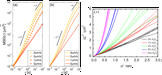
\includegraphics[width=0.85\textwidth]{figures/msdmicroscopicagents.pdf}
  \end{center}
  \caption[MSD for brownian particles]{MSD for brownian particles with different velocites. \textbf{Panel a)} shows the result from simulations. \textbf{Panel b)} shows the theoretical calculation, obtained from~\cite{volpe2014simulation}. \textbf{Panel c)} MSD for different velocities of polystyren spheres for different concentrations of Hydrogen Peroxide, obtained from~\cite{howse2007self}.}\label{fig:msddifferentvelocities}
\end{figure}

Tierno et al. (2008) proposed a new mechanism where two linked paramagnetic colloidal particles of different sizes, need no deformation for propulsion~\cite{tierno2008controlled}. Their setup consists of colloids dispersed in water above a flat glass plate in the presence of a precessing magnetic field parallel to the plate. Here, the plate plays an important role for the rotating colloids, due to the dynamics it has when particles are near a boundary. When the smaller one is near the glass, the viscosity increases, resulting in lateral translation of the small colloid.


Based on the premise of biomedical purposes, Ghosh et al. (2009) proposed a system where helical screw nano propellers' control is so precise that it can be manipulated with a tolerance of microns~\cite{ghosh2009controlled}. Their size is approximately 200-300 nm, making them ideal for navigating confined spaces inside and not being intrusive. They are driven by a magnetic field. Half of the helices are covered with cobalt, which has ferromagnetic properties, and then placed between two electromagnetic poles with a homogeneous precessing magnetic field, making the magnetic moment align with their long axis. Since the ferromagnetic part has a natural magnetic moment, it aligns with the external field, causing it to rotate along the helix. For each rotation, the particle moves either forward or backward, depending on certain values of the helix's geometry. 

\subsection{Natural Systems}

We note how researchers have developed numerous strategies to achieve what was already accomplished by nature over a long period. In this section, we will present some examples of biological agents that inspired this thesis.

 In a research by Corkidi et al. (2008) spermatozoa behavior was studied in a 3-dimensions space mimicking their real environment in searh for eggs, what they found was a helical trajectory, shown in Figure~\ref{fig:corkidiexperiment}, being a pretty similar response, and obtaining a non-space dependant behavior~\cite{corkidi2008tracking}. 

\begin{figure}[h]
  \begin{center}
    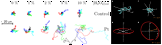
\includegraphics[width=0.90\textwidth]{figures/randomwalk.pdf}
  \end{center}
  \caption[Random Walk for active brownian particles.]{Trajectories of polystyren platinum layered sphere particles for different peroxide consentrations, obtained from~\cite{howse2007self}.Trajectory of the spermatozoa for \textbf{a,c} free space, and \textbf{b, d} confined 2-dimension space. Obtained from~\cite{corkidi2008tracking}.}\label{fig:corkidiexperiment}
\end{figure}



It seems we cannot avoid randomness even for active particles, in a regime where viscous forces are predominant, a little symmetry breaking noise that perturbs the direction of the particle can make the origin of a random walk, but nature, as always, has evolved elegant solutions to this challenge through various biological mechanisms. A prime example is E. coli, which employs helical flagella that can rotate both clockwise and counterclockwise, generating two distinct types of motion that researchers have termed "run"—swimming in a straight line—and "tumble"—rotation in a random direction. This behavior also depends on the medium's viscosity and random fluctuations~\cite{kumar2010physics}. The way E. coli achieves a "run" state is due to their flagella which has two different motions for its power and recovery strokes, simulating those of a human breast strokes, although a tumble state is unavoidable, it is a great opportunity to harness the directed motion of the particle and see if it is possible to obtain work of it. 


Marine bacteria are another example of an organic microswimmer; this can obtain individual speeds ten times faster than that of E. Coli (40 $\mu m s^{-1}$)~\cite{mitchell1995long, lowe1987rapid}. Marine bacteria have a similar mechanism as E. Coli, responding to amino acids utilising a run and reverse motion, different from the run and tumble, allowing them to stop and reverse their directon, making it more efficient reaction~\cite{barbara2003marine}. However, since this bacterium is often found in the ocean, where its nutrients are constantly in motion, a study by Barbara et al. (2002) aimed to investigate how it would react to obtain its nutrients~\cite{barbara2003bacterial}. Interestingly, thanks to the motion system, marine bacteria were able to turn multiple times in the direction of the nutrients, thereby tracking them unequivocally.

Another remarkable example of biologically active matter is the green alga \textit{Chlamydomonas reinhardtii}. This unicellular microorganism swims using two anterior flagella that beat in a breaststroke-like motion, propelling the cell forward through the water. Unlike bacteria, which rotate their helical flagella, \textit{Chlamydomonas} relies on the coordinated motion of paired flagella, leading to straight swimming when both are synchronized and to turning when the coordination is lost~\cite{goldstein2015green}. Because of this, \textit{Chlamydomonas} is often used as a model organism to understand how eukaryotic cells achieve motility at low Reynolds number.

Another type of biological microswimmer is found in protozoa such as \textit{Paramecium}. These ciliates are covered with thousands of cilia that beat in a coordinated manner, producing smooth gliding motion through viscous fluids~\cite{zhang2015paramecia}. Cilia not only enable propulsion but also allow \textit{Paramecium} to sense and respond to chemical gradients in their environment, demonstrating an early form of mechanosensory feedback in microswimmers.

At a different scale, immune system cells, such as neutrophils, also display active motility, although they crawl rather than swim. Neutrophils move by extending actin-rich protrusions (lamellipodia) and contracting their cell body, enabling them to pursue pathogens in tissues~\cite{friedl2004collective}. While their propulsion mechanism differs from that of flagellated or ciliated organisms, neutrophils still exemplify how living systems consume energy internally to generate directed motion.

These diverse biological strategies demonstrate how nature has evolved multiple solutions to achieve motion in environments dominated by viscous forces. Each of these mechanisms—flagellar beating in algae, ciliary coordination in protozoa, or actin-driven crawling in immune cells—highlights the central role of active matter principles in biology. But, is their locomotion enough to produce work?

\section{Obtaining Work from Active Matter}

A fundamental question in active matter research is whether the continuous energy consumption and motion of biological microswimmers can be harnessed to perform useful work. In nature, molecular motors such as kinesin, dynein, and myosin already accomplish this inside cells, driving processes like vesicle transport, muscle contraction, and chromosome segregation. Inspired by these nanoscale examples, researchers have investigated whether intact organisms at the microscale can be used as biological engines outside their natural environments~\cite{schliwa2003molecular}.

One particularly illustrative example comes from the work of Weibel et al. (2005), who introduced the concept of \textit{``microoxen''} --- motile cells of the green alga \textit{Chlamydomonas reinhardtii}~\cite{weibel2005microoxen}. In their study, the authors exploited the flagellar beating of \textit{Chlamydomonas} to transport microscale loads such as polystyrene beads. By chemically attaching the beads to the cell wall, these algae were able to carry particles 1--6 µm in diameter without significantly reducing their swimming velocity (100–200 µm/s, similar to unmodified cells). 

An important feature of this work was the ability to control and manipulate the cells. Because \textit{Chlamydomonas} exhibits positive and negative phototaxis~\cite{bennett2015steering}, its direction of motion could be guided in microfluidic channels by alternating visible light sources. This allowed them to steer cargo-carrying cells back and forth repeatedly over distances of up to 20~cm. Moreover, by including a \textit{photocleavable chemical linker} between the load and the cell surface, they enabled the controlled release of particles using UV light, allowing cells to pick up, transport, and drop off cargo on demand.

This study highlights served as inspiration for using living active matter to perform mechanical work. On one hand, it demonstrates that whole microorganisms can act as microscopic carriers, and self-sustaining energy supply. On the other hand, it also underscores practical limitations: maintaining living cells, and preventing adhesion to surfaces.

 Qin et al. (2007) attempted to harness the dynamics of the decomposition of previously studied hydrogen peroxide, but rather than creating a system of linear motion, they employed it in a different manner. It is a similar approach as the nanorods, that use stripes of Pt and Au, this time they use a small surface, ressembling a path in one part of the rod, this configuration makes the release of oxygen bubbles in a lateral being capable of producing torque on the rod and therefore making it spin, thanks to this, they were able to create a nanorotor~\cite{qin2007rational}. However, we can argue that they are not harnessing the behavior of active matter to create work, but rather making active matter behave a certain way.

 \begin{figure}[h]
  \begin{center}
    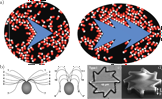
\includegraphics[width=0.95\textwidth]{figures/harnessWork.pdf}
  \end{center}
  \caption[Experiments that harness bacteria motility.]{Expermients that harness bacteria motility. \textbf{Panel 1)} shows how the bacteria accumulates in the concave sections of the shuttle, finally aligning parallelly, obtained from~\cite{angelani2010geometrically}. \textbf{Panel 2} drawing of Chlamydomonas reinhardtii's movement, obtained from~\cite{weibel2005microoxen}. \textbf{Panel 3) - 4)} shows an example of ratchet used in experiments, made by lithography, obtained from~\cite{di2010bacterial}.}\label{fig:harnesswork}
\end{figure}

Another novel demonstration of obtaining work from active matter was presented by Hiratsuka et al. (2006), who developed a microrotary motor powered by the gliding bacterium \textit{Mycoplasma mobile}~\cite{hiratsuka2006microrotary}. Unlike flagellated swimmers \textit{E. coli} or \textit{Chlamydomonas}, \textit{M. mobile} moves by gliding over solid surfaces at speeds of 2–5 µm/s, using sialic proteins in the surface of the track. The authors harnessed this motility by integrating living cells into lithographically fabricated microdevices.

Their microrotary motor consisted of a circular silicon track, into which \textit{M. mobile} cells were guided asymmetrically so that the majority moved in a unidirectional loop. A 20 µm silicon dioxide rotor with protrusions that fit into the circular track was then docked, and cells were chemically linked to its surface via biotin–streptavidin interactions. As the bacteria glided along the track, they pulled the rotor, producing unidirectional rotation at rates of 1.5–2.6 revolutions per minute (rpm). The torque generated by individual cells was estimated to be $2$–$5\times10^{-16}$ N·m, sufficient to overcome viscous drag at the microscale.

This work represents a successful integration of living motile cells with inorganic micromachinery, demonstrating that whole microorganisms can be harnessed to drive artificial devices. 


Angelani et al. (2010) noticed how asymmetric geometry can be used to harness the randomness of particles to obtain work from them. Using numerical simulations, they mimicked elongated motile bacteria, and the object to move consisted of an arrow-shaped structure with a varying number of teeth, ranging from 2 to 8. They saw that some particles get trapped between the spaces of the teeth, aligning themselves, making it possible to push the \textit{shuttle}, and due to dynamics, they eventually get unstuck and return to swim free in the solution. The simulations were performed in 2 dimensions, where bacteria were able to push the object~\cite{angelani2010geometrically}.

Beyond the use of single microorganisms as engines, researchers have also looked at how collective active matter might be used to produce work. Thampi et al. (2016) showed in simulations that dense active fluids—like bacterial suspensions or mixtures of microtubules with motor proteins—can display mesoscale turbulence that can be rectified to move micromachines~\cite{thampi2016active}.

In their setup, a square array of symmetric microrotors was placed inside an active nematic fluid. Although the rotors were geometrically identical, the system broke symmetry on its own: neighboring discs settled into an alternating spin pattern, rotating in opposite directions. In this way, disordered turbulent flows were turned into a regular and steady source of rotation. The extent and stability of the rotation depended on rotor size and spacing, with the best results when the separation was comparable to the natural vortex size of the active turbulence.

This study is useful here for two reasons. First, it shows that work can be obtained from active turbulence without introducing asymmetry or applying external fields. Second, it illustrates how geometry and confinement help stabilize active flows—ideas that will be relevant again in this thesis when we study colloids and ratchet systems under external driving.

A central question in active matter is how to harness the continuous energy consumption of self-propelled agents to perform useful work. Inside cells, proteins such as kinesin and dynein already fulfill this role at the nanoscale, but the prospect of exploiting entire microorganisms as microscopic engines is especially appealing. Early studies demonstrated that bacteria could be attached to synthetic objects and used to propel them forward~\cite{weibel2005microoxen, hiratsuka2006microrotary}. The resulting motion, however, was generally random.

A major advance came with the work of Di Leonardo et al. (2010), which served as inspiration for this thesis, showing that geometry alone can guide bacterial motion without the need for external fields~\cite{di2010bacterial}. In their experiments, sawtooth-shaped microgears with diameters of approximately 48~µm were immersed in dense suspensions of motile \textit{E. coli}. The bacteria accumulated and aligned at the concave corners of the gears, collectively exerting a torque that rotated the structures. At cell concentrations on the order of $10^{10}$~mL$^{-1}$, the gears achieved steady angular velocities of about 2~rpm. This behavior follows the mechanism described by Angelani et al. (2010), where cells become transiently trapped between the asymmetric teeth, pushing against the walls and generating directed motion~\cite{angelani2010geometrically}. 

Interestingly, the authors also tested different geometries. As expected, asymmetric rotors produced net rotation, while symmetric ones yielded zero average angular velocity, underscoring the importance of symmetry breaking in rectifying bacterial motion. 

This result demonstrates that combining bacterial activity with asymmetric boundaries can act as a ratchet, transforming random fluctuations into directed motion. The concept recalls the Feynman ratchet thought experiment, but here it is realized in a living system, powered solely by bacterial metabolism. Such bacterial ratchets not only provide fundamental insight into nonequilibrium statistical mechanics but also suggest potential applications in microfluidics, where pumps and mixers could operate autonomously without external energy inputs.

\chapter{Magnetically Driven Colloidal Systems}
\label{magneticallydrivencolloidalsystems}


We can see that biological active matter is effective at transporting or moving objects. The drawback, however, is that these systems always require a constant supply of energy. So far, there is no unlimited energy source available for this purpose. An exception are thermophoretic particles, which only need a beam of light to create a temperature gradient. In fact, some experiments have combined this principle with machine learning models, allowing particles to be guided toward a target region while reducing the impact of thermal noise~\cite{muinos2021reinforcement}. The limitation, though, is that only a relatively small number of particles can be manipulated in this way, which is not enough to drive something like a rotor.

Because of this, we take a different approach. The idea is to combine active and passive matter, so that energy can be injected into the system without having to replace the entire source each time. This hybrid strategy may offer a way to overcome the limits seen in purely biological or purely synthetic setups.

This thesis focuses on paramagnetic colloids. Their key property is that the magnetic dipoles align with an external field, but once the field is removed, the dipoles lose their orientation and the material no longer shows magnetic order. The origin of this effect lies in the electronic and spin configuration of the atoms. A simple example is molecular oxygen, $O_2$, which has two unpaired valence electrons with the same spin. This imbalance leads to a net magnetic moment, giving rise to paramagnetism. The underlying principle is explained by Hund’s rule.

By themselves, paramagnetic particles cannot be considered active matter, even in the presence of a magnetic field. Several experiments have tried to induce motion in these systems, and one promising route is through Brownian rectification. For example, Tierno (2012) studied paramagnetic colloids placed above a ferrite garnet film. The film contained permanent magnetic domains aligned along the $x$-axis, with alternating directions, while the colloids were subjected to a circularly precessing magnetic field in the $y$–$z$ plane~\cite{tierno2012depinning}.

With these parameters, and by varying only the driving frequency, four regimes of motion were identified. At the highest frequencies, the particles entered a pinned state, meaning the colloids did not translate. Tierno also tested elliptic magnetic fields and observed that, depending on the field magnitude, the particles displayed either attractive or repulsive interactions. These behaviors arise from the dipole–dipole potential between particles, given by

\begin{equation}
U_{dd} = \frac{\mu}{4\pi} \left( \frac{m_i m_j}{r^3_{ij}} - \frac{3(m_i \cdot r_{ij})(m_j \cdot r_{ij})}{r^5_{ij}} \right),
\label{eq:dipolepairpotential}
\end{equation}

where $m_i$ and $m_j$ are the magnetic moments of particles $i$ and $j$, and $r_{ij}$ is their separation vector.

A subsequent study by Straube and Tierno (2013) provided a deeper understanding of these dynamics by analyzing the role of synchronization and thermal noise~\cite{straube2013synchronous}. Using the same ferrite garnet film with periodic magnetic domains, they investigated the motion of a single paramagnetic colloid driven by a rotating magnetic field. At low driving frequencies, the particle remained synchronized with the moving magnetic potential, resulting in constant-speed transport at the same velocity as the traveling landscape. Above a critical frequency, however, the particle lost synchronization, entering an asynchronous regime characterized by intermittent sliding and a reduced average speed.

To describe these results, Straube and Tierno proposed a simplified analytical model based on the overdamped Langevin equation, which accounted for both deterministic forces and thermal fluctuations. Importantly, their model showed excellent agreement with experiments and revealed how thermal noise smooths the sharp transition between synchronous and asynchronous regimes. This highlights the interplay between deterministic driving and stochastic forces in rectification phenomena, and demonstrates how even passive colloids can be controlled and transported through external fields when symmetry is broken.

A year later, they used the same system with a rotating magnetic field whose ellipticity could be tuned~\cite{straube2014tunable}. The effect of this field was to create an asymmetric traveling potential that rectified Brownian motion and transported the particles across the surface.

One of the main results was that the interaction between particles could switch from repulsive to attractive just by adjusting the ellipticity of the field. In the attractive case, particles came together into stable doublets that moved with constant velocity along the magnetic stripes. They measured the dipolar forces that caused this binding and proposed a model that matched well with the experiments.

This shows that not only single-particle motion can be controlled, but also collective effects like chain formation and cooperative transport. The fact that this can be tuned with an external field suggests possible uses in microfluidics or lab-on-chip devices, where clustering or separation of particles can be useful for transport, mixing, or sorting.

This dipole-dipole attractive and repulsive interaction between particles, is a key aspect for this thesis. More recently, Stoop et al. (2021) studied a dense monolayer of paramagnetic colloids driven above a triangular lattice of magnetic bubbles using a rotating magnetic field~\cite{stoop2020collective}. The external field generated a two–dimensional traveling wave ratchet that transported the particles across the substrate. While single colloids showed no preferred direction of motion, collective interactions at higher densities led to a spontaneous symmetry breaking. In this regime, the particle current locked along one of the crystallographic axes of the lattice, producing a transversal current even though the driving direction was set between two symmetry axes.

They also reported that this locking could be polarized by adding a weak bias field, which made one direction energetically favorable over the other. At intermediate densities, elongated clusters of particles formed and moved coherently, showing that dipolar interactions stabilize directional locking. At very high densities, however, the effect was lost as the colloids formed a percolating network covering the entire substrate.

This work highlights how collective effects can generate robust directional transport that does not appear at the single-particle level. It shows that by controlling density and external fields, transport in colloidal systems can be tuned or polarized, which is useful for applications such as particle sorting and microfluidic control. 


%%%
A recent study by Ostinato \textit{et al.} (2024) explored the collective dynamics of paramagnetic colloids confined between two plates separated by less than twice the particle diameter and driven by a precessing magnetic field~\cite{ostinato2024magnetically}. Using numerical simulations, they demonstrated that the interplay between confinement and dipolar interactions can produce two distinct transport regimes.

When the applied precessing field was spatially isotropic, the particles did not display a net current but instead showed enhanced diffusion, with an effective diffusion coefficient up to 60 times larger than that of unforced colloids. This enhancement originated from a continuous exchange of positions between colloids near opposite walls, a motion resembling a ``ceilidh dance'' of dimers that bind and unbind periodically \cite{ostinato2024magnetically}. 

In contrast, introducing a small spatial anisotropy by tilting the precession axis ($\delta \neq 0$) generated a robust bidirectional current. In this regime, colloids organized into two parallel flows moving in opposite directions, achieved by synchronized particle exchanges across the two planes. The magnitude of this current was highly tunable by varying both the driving frequency and the tilt angle, reaching maximal values when particles jumped exactly one lattice constant per field cycle. Remarkably, this bidirectional transport was robust against single-particle defects but could be disrupted by the introduction of ``magnetic holes'' (nonmagnetic inclusions in the ferrofluid), which acted as localized defects that broke the current pathways.

These results provide a powerful demonstration of how geometrical confinement and external field anisotropy can convert random thermal motion into ordered transport, without the need for field gradients. They highlight new opportunities for designing microfluidic devices where colloids could be directed, mixed, or sorted by simply tuning the parameters of an external homogeneous field.

%%%
\newpage
